\chapter{Kravspecifikation}
Ud fra projektformuleringen er der formuleret en række krav til projektet. Disse indebærer to use cases og et antal ikke-funktionelle krav. Følgende afsnit beskriver aktøren for systemet samt de krav der er sat til systemet.

\section{Aktørbeskrivelse}
På figur \ref{fig:useCaseDiagram} ses use case diagrammet for systemet. På figuren ses det at der er én primær bruger for systemet, brugeren. 

\begin{figure}[H]
	\centering
	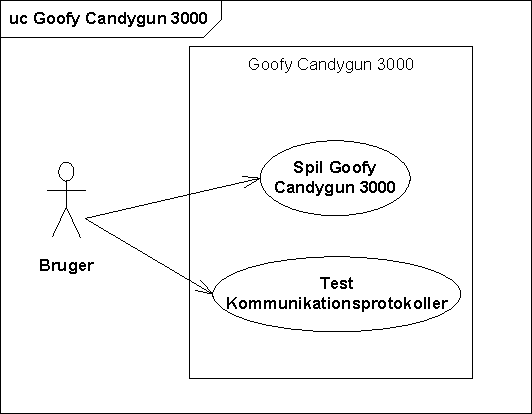
\includegraphics[width=0.80\textwidth]{Kravsspecifikation/images/usecaseDiagram}
	\caption{Use case diagram}
	\label{fig:useCaseDiagram}
\end{figure}



\subsection{Aktør - Bruger}

\begin{tabularx}{\textwidth}{| p{2cm} | p{9.1cm} |}
	\hline
	Aktørens Navn: & Bruger \\ 
	\hline
	Alternativ Navn: & Spiller \\
	\hline
	Type: & Primær \\
	\hline
	Beskrivelse: & Brugeren initierer Goofy Candygun 3000 samt starter systemtesten. Derudover har brugeren mulighed for at stoppe spillet igennem brugergrænsefladen. Brugeren vil under spillet interagere med Goofy Candy Gun gennem Wii-Nunchucken.
	\\ \hline
\end{tabularx}

\newpage
\section{Use case beskrivelse}
I dette afsnit følger en beskrivelse af de to use cases og de ikke-funktionelle krav, som er defineret i \textbf{\#ref reference til kravspecifikationen i Dokumentationen.}
\subsection{Use case 1}
Brugeren initierer use casen ved at starte spillet via brugergrænsefladen og vælge spiltype; oneplayer eller partymode. Herefter vælges antallet af skud i et spil og disse puttes i magasinet. Når dette er gjort kan spillet påbegyndes. Brugeren indstiller kanonen med Wii-nunchuck og affyrer den. Herefter lader systemet et nyt skud og samme procedure gentages. Til slut vises information om spillet på brugergrænsefladen, brugeren afslutter spillet ved at trykke på knappen på brugergrænsefladen og denne vender tilbage til starttilstanden. 

\subsection{Use case 2}
Brugeren initierer use casen ved starte systemtesten via brugergrænsefladen. Herefter testes forbindelserne mellem hardwareblokkene forbundet via systemets busser. Hvis der sker fejl under systemtesten, raporteres disse til brugeren via brugergrænsefladen og use casen afbrydes. Ved en successfuld systemtest, rapporteres dette til brugeren via brugergrænsefladen og systemet er klar til brug.

\section{Ikke-funktionelle krav}
Til beskrivelse af produktets specifikationer er der udarbejdet nogle ikke-funktionelle krav. Disse sætter krav til systemets og projektilers dimensioner. Derudover sættes der en begrænsning til kanonens rotation, samt krav til afvikling af kanonens udløsning.  








